\section{Appendix - Raw Data}

\begin{figure}[hbtp]
  \centering
  \caption{Results gathered from the first test run}
  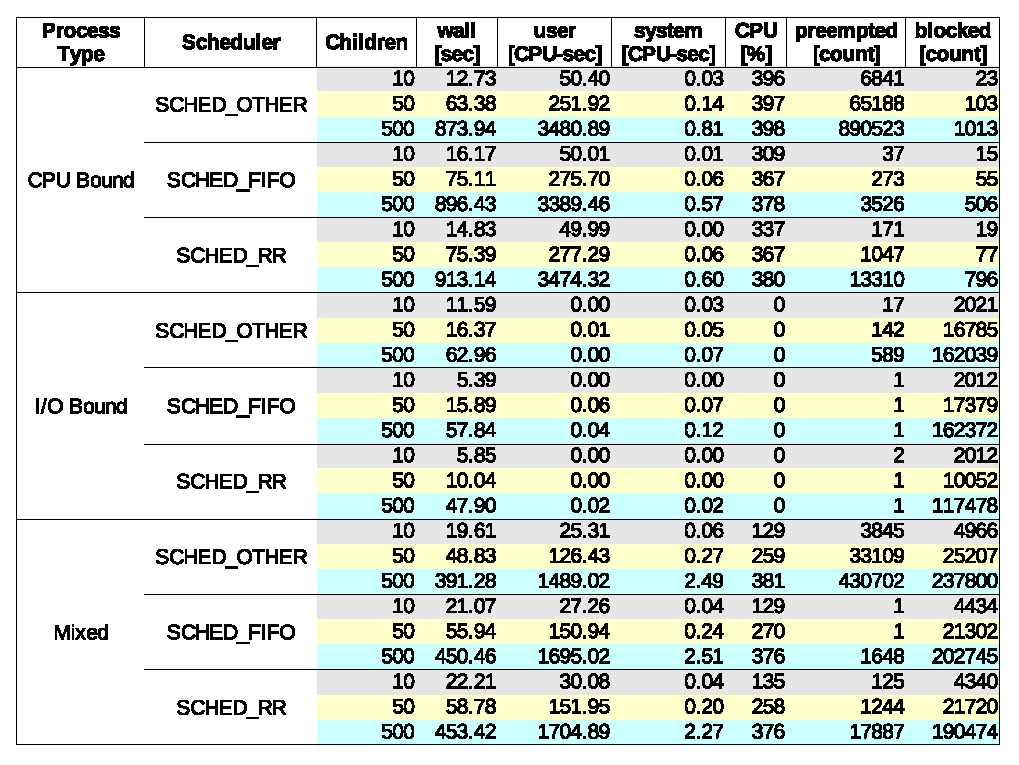
\includegraphics[scale=1.0]{img/raw-results1-table.eps}
  \label{tab:raw-results1}
\end{figure}

\begin{figure}[hbtp]
  \centering
  \caption{Results gathered from the second test run}
  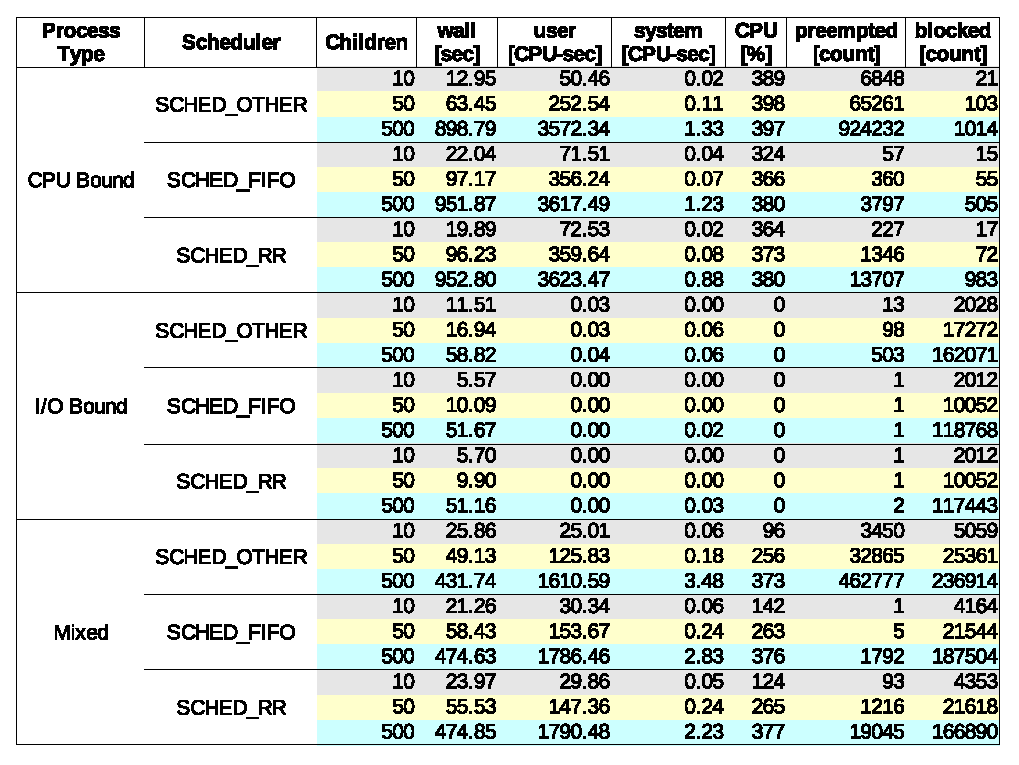
\includegraphics[scale=1.0]{img/raw-results2-table.eps}
  \label{tab:raw-results2}
\end{figure}

\begin{figure}[hbtp]
  \centering
  \caption{Results gathered from the third test run}
  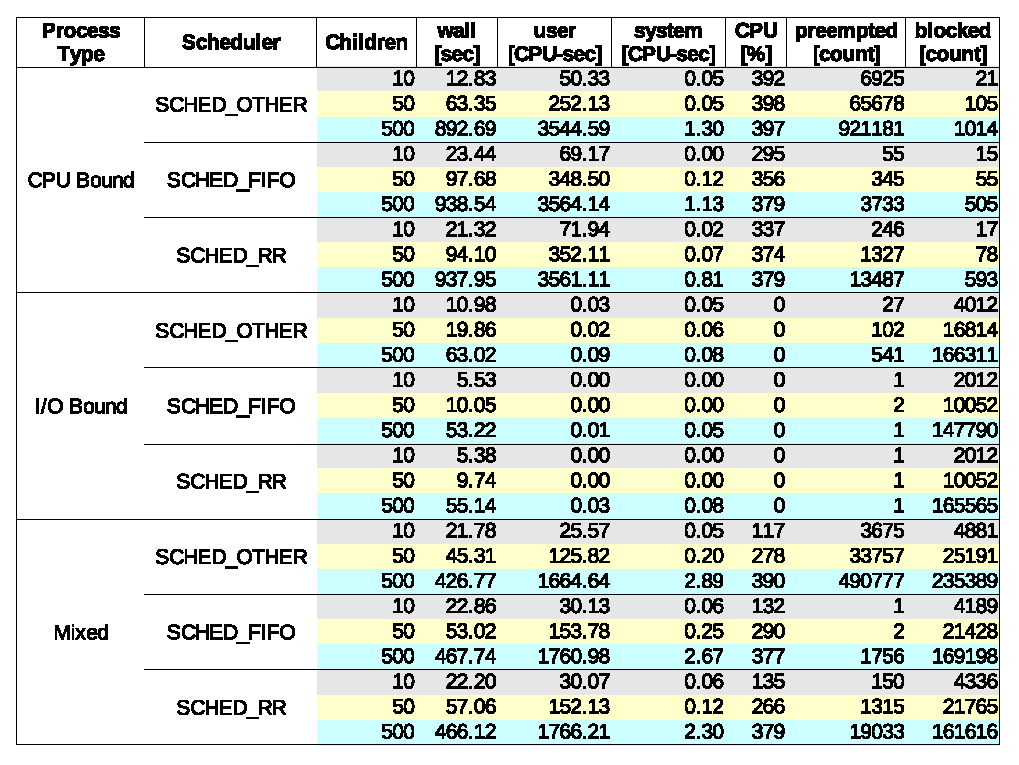
\includegraphics[scale=1.0]{img/raw-results3-table.eps}
  \label{tab:raw-results3}
\end{figure}

\begin{figure}[hbtp]
  \centering
  \caption{Averaged results over all three test runs}
  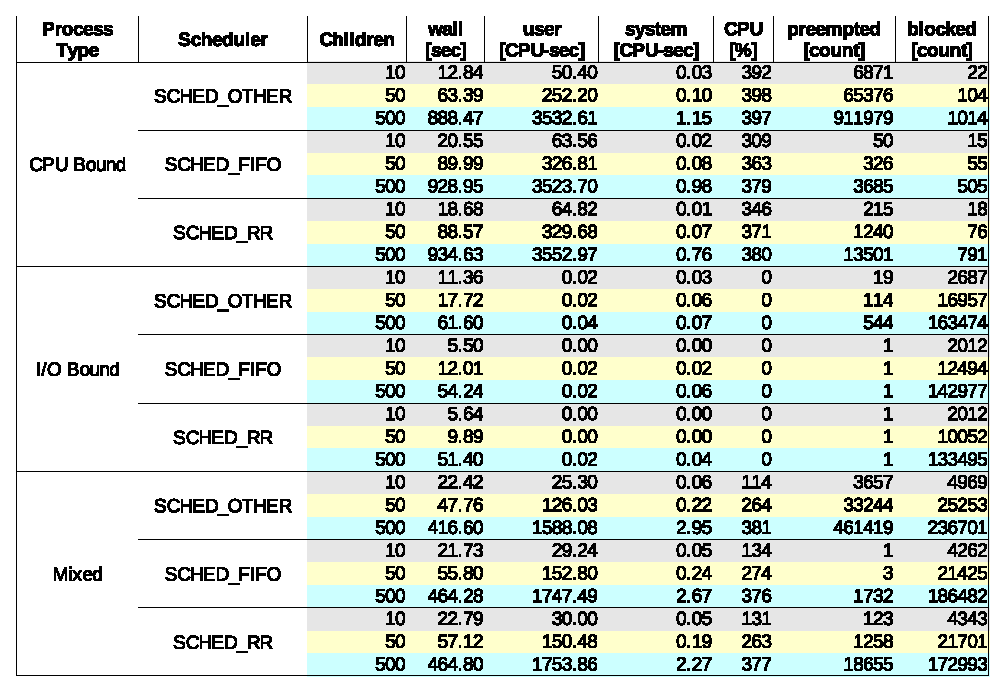
\includegraphics[scale=1.0]{img/raw-results-table.eps}
  \label{tab:raw-results}
\end{figure}

\begin{figure}[hbtp]
  \centering
  \caption{Averaged results over all three test runs, divided by the respective number of child processes}
  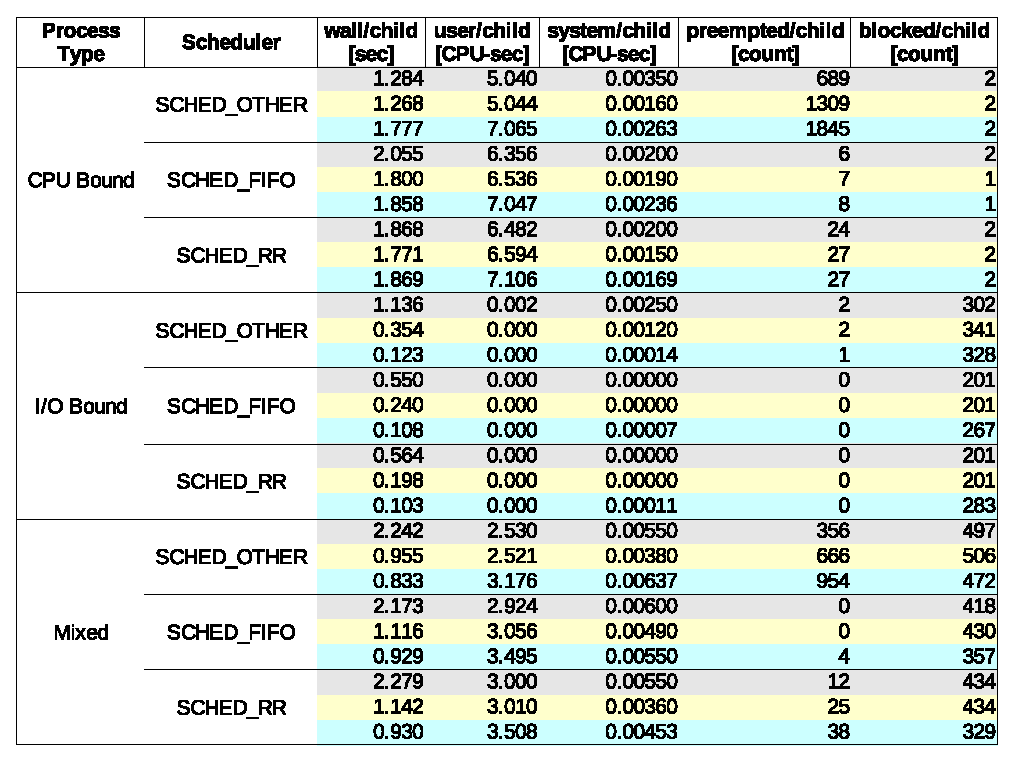
\includegraphics[scale=1.0]{img/raw-results-child-table.eps}
  \label{tab:raw-results-child}
\end{figure}

